\title{Adaptive data-driven age and patch mixing in contact networks with recurrent mobility}
\author[1,2,a,*]{Jesse~Knight}
\author[1,b]{Huiting Ma}
\author[3]{Amir Ghasemi}
\author[1,d]{Mackenzie Hamilton}
\author[4,5,e]{Kevin Brown}
\author[1,2,5,6,f]{Sharmistha Mishra}
\affil[1]{MAP Centre for Urban Health Solutions, Unity Health Toronto}
\affil[2]{Institute of Medical Science, University of Toronto}
\affil[3]{Communications Research Centre Canada, Ottawa}
\affil[4]{Public Health Ontario, Canada}
\affil[5]{Dalla Lana School of Public Health, University of Toronto}
\affil[6]{Division of Infectious Diseases, Department of Medicine, University of Toronto}
\affil[a]{ORCID: 0000-0002-0455-5455}
\affil[b]{ORCID: 0000-0003-1910-5614}
%\affil[c]{ORCID: }
\affil[d]{ORCID: 0000-0003-2423-3629}
\affil[e]{ORCID: 0000-0002-1483-2188}
\affil[f]{ORCID: 0000-0001-8492-5470}
\affil[*]{Corresponding Author: Jesse Knight.
  \texttt{jesse.knight@mail.utoronto.ca}}
\date{Sept 26, 2021}
\keywords{%
  COVID-19,
  Mathematical modelling,
  Heterogeneous mixing,
  Population mobility
}
\abstract{Infectious disease transmission models often stratify populations by age and geographic patches.
Contact patterns between age groups and patches are key parameters in such models.
Arenas et al.\ (2020) develop an approach to simulate contact patterns associated with
recurrent mobility between patches, such as due to work, school, and other regular travel.
% JK: @SM added next sentence based on suggestion in 3.2 Results.
%     I have mixed feelings about it, because I think is an important point,
%     but might slightly interrupt the flow of ideas, and not sure where else to put it.
% SM: I like including this too. it didn't feel like an interruption in flow. made a few edits for consideration to suggest this point is also part of the 'results' of the paper (vs. what has already been shown?)
First, we demonstrate that using their approach, mixing between patches is greater than mobility data alone would suggest,
because individuals from patches A and B can form a contact if they meet in patch C.
We then build upon their approach to address three potential gaps that remain.
First, our approach includes a distribution of contacts by age
that is responsive to underlying age distribution of the mixing pool.
Second, different age distributions by contact type are also maintained in our approach,
such that changes to the numbers of different types of contacts
are appropriately reflected in changes to the overall age mixing patterns.
Finally, we introduce and distinguish between two mixing pools associated with each patch,
with possible implications for the overall connectivity of the population:
the home pool, in which contacts can only be formed with other individuals residing in the same patch;
and the travel pool, in which contacts can be formed with some residents of, and any other visitors to the patch.
We describe in detail the steps required to implement our approach,
and present results of an example application.
}
\grabstract{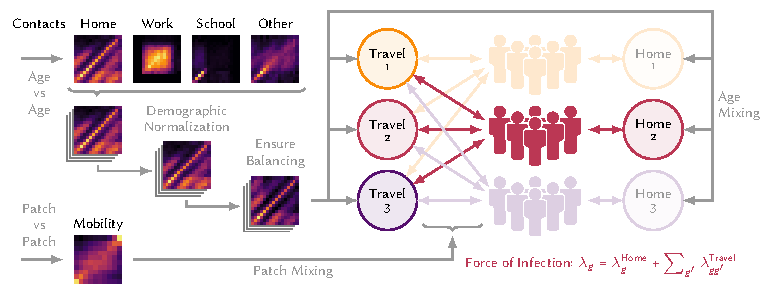
\includegraphics[width=\linewidth]{grabstract}}
\submission{Direct}
\area{Bioinformatics}
\subject{Epidemic modelling}
\method{\fullcite{Arenas2020}}
\resource{\hreftt{https://github.com/mishra-lab/mobile-patch-mixing}}
\funding{%
  The study was supported by:
  the Natural Sciences and Engineering Research Council of Canada (NSERC CGS-D);
  the Canadian Institutes of Health Research (VR5-172683); and
  the 2020 COVID-19 Centred Research Award from the St Michael's Hospital Foundation Research Innovation Council.}
\acknowl{%
  We thank:
  Kristy Yiu (Unity Health Toronto) for research coordination support;
  Gary Moloney (Unity Health Toronto) for support with geographic data processing and helpful discussions; and
  Linwei Wang (Unity Health Toronto) for helpful discussions.
  \par
  Reported \covid cases were obtained from
  the Public Health Ontario (PHO) integrated Public Health Information System (iPHIS),
  via the Ontario \covid Modelling Consensus Table,
  and with approval from the University of Toronto Health Sciences REB (protocol No.~39253).
}
\contrib{%
  JK conceived of and developed the approach, reviewed the literature, conducted the mixing and mobility analyses, and wrote the code and manuscript.
  AG conducted and led data analyses and developed the mobility metrics.
  HM provided critical input into the assumptions and bias adjustments with the mobility data.
  MH, KB, and SM contributed critical insights to the assumpitons, data, approach, and interpretation.
  All authors were involved in intepretation and manuscript revisions.
}